% 10 pages, excluding references
% Abstract 05/12
% Paper 12/12
% CCGrid will be following a double-blind review process
% IEEE two-column conference proceedings template

\documentclass[conference,10pt]{IEEEtran}

\def\BibTeX{{\rm B\kern-.05em{\sc i\kern-.025em b}\kern-.08em
    T\kern-.1667em\lower.7ex\hbox{E}\kern-.125emX}}

\usepackage[utf8]{inputenc}
\usepackage{amsmath, amssymb, amsfonts, colortbl, xspace, todonotes, paralist, multirow, hyperref, pgfplots}
\pgfplotsset{compat=newest}
\hypersetup{
   colorlinks=false,
   pdfborder={0 0 0},
}
\usepackage[english]{babel}
\usepackage{graphicx, color, amssymb, url, xcolor, tikz, pgf, float, subcaption, algorithm,  tabularx}
\usepackage[noend]{algpseudocode}
\usetikzlibrary{trees, shapes, calc, external, fit, arrows, decorations, decorations.pathreplacing, patterns, automata, positioning, arrows.meta, intersections, calligraphy}

% Custom commands
\algnewcommand\algorithmicforeach{\textbf{for each}}
\algdef{S}[FOR]{ForEach}[1]{\algorithmicforeach\ #1\ \algorithmicdo}
\renewcommand{\algorithmicrequire}{\textbf{Input:}}
\renewcommand{\algorithmicensure}{\textbf{Output:}}
\newcommand{\Node}[1]{\ensuremath{\mathrm{Node}_{#1}}\xspace}
\newcommand{\flow}[1]{\ensuremath{\mathit{flow}_{#1}}\xspace}
\newcommand{\file}{\ensuremath{\mathit{File}}\xspace}
\newcommand{\storage}{\ensuremath{\mathit{Storage}}\xspace}
\newcommand{\memory}{\ensuremath{\mathit{Mem}}\xspace}
\newcommand{\memorymap}{\ensuremath{\mathcal{M}_{map}}\xspace}
\newcommand{\duration}{\mathit{Duration}\xspace}
\newcommand{\bandwidth}{\mathit{BW}\xspace}
\newcommand{\core}{\mathit{Cores}\xspace}
\newcommand{\submissiontime}{\mathit{Subtime}\xspace}
\newcommand{\walltime}{\mathit{Walltime}\xspace}
\newcommand{\completiontime}{\mathit{Completiontime}\xspace}
\newcommand{\start}{\mathit{Starttime}\xspace}
\newcommand{\fileset}{\ensuremath{\mathbb{F}}\xspace}
\newcommand{\jobset}{\ensuremath{\mathbb{J}}\xspace}
\newcommand{\nodeset}{\ensuremath{\mathbb{N}}\xspace}
\newcommand{\evict}{\ensuremath{\mathcal{V}}\xspace}
\newcommand{\nbloads}{\ensuremath{\mathit{\mathit{Loads}}}\xspace}
\newcommand{\live}{\ensuremath{L}\xspace}
\renewcommand{\algorithmicrequire}{\textbf{Input:}}
\renewcommand{\algorithmicensure}{\textbf{Output:}}

\begin{document}

\title{Locality-aware batch scheduling of I/O intensive workloads}

\maketitle


\begin{abstract}	
  Clusters and supercomputers make use of workload schedulers such as
  the Slurm Workload Manager 
  % or OAR 
  to allocate computing jobs onto nodes. These schedulers
  usually aim at a good trade-off between increasing resource
  utilization and user satisfaction (decreasing job waiting
  time). However, these schedulers are typically unaware of jobs
  sharing large input files: in data-intensive scenarios,
  tens to hundreds of jobs dedicated to the study of the same multi-GB input
  file may be successively submitted, leading to a large data transfer overhead. 
  
  % Running each of these jobs first requires to load the input file, leading to a large data transfer overhead. 
  
  
  % Users could manually group some of these tasks into larger jobs to reduce data transfers, but this would result in less granular units that are more difficult to schedule by the resource manager, and would thus result in a larger delay as well.
  
  
  We study how to design a \textit{data-aware
  job scheduler} that is able to keep large input files on the 
  computing nodes, 
  % provided this does not impact the memory needs of other jobs, 
  without impacting other memory needs,
  and can use previously loaded files to \textit{limit
  data transfers in order to reduce the waiting times of jobs}.

  We present three schedulers capable of distributing the load between
  the computing nodes as well as 
  % being aware of what the memory of each node contains in order to re-use an input file
  re-using an input file
  % already loaded in the memory of some node as many times as possible.
  already loaded in the memory of some node as much as possible.
  
  % We report simulations performed using real cluster usage traces. 
  We perform simulations using real cluster usage traces. 
  % Our approach is compared to currently used schedulers in batch systems.
  % The results show that keeping data locally, in memory, between successive
  The results show that keeping data locally, between successive
  jobs and using data locality information to schedule jobs allows a
  reduction in job waiting time and a drastic decrease in the amount of data
  transfers.
  
    %~ \todo[inline]{Max: Should we explicit the "Simple Linux Utility for Resource Management"?LM: I think it's fine in the abstract, we give a reference below. Max: Okay. Carl: I believe the SLURM project itself is claiming it's not an acronym for that anymore. The proper name is the "Slurm Workload Manager".}
	%~ \todo[inline]{Max: Should we precise that it's in certain areas of research that you are really highly data-dependent? LM: maybe again give details about this in the introduction. Max: alright.}
	%~ \todo[inline]{Max: Should we talk about our competitors FCFS and EFT
	%~ with and without backfilling? Sam: we can say that we compare with
	%~ schedulers currently used by job schedulers. Max: Okay, I added a sentence.}
\end{abstract}

%~ \todo[inline]{LM: I changed memory into storage: is it correct ? Carl: I changed back, the point is that these large files are kept in memory with heavy random accesses. There are of course cases where local scratch is sufficient for random accesses, but this not the scenario we've been focusing on. Changed it back.}

\begin{IEEEkeywords}
%~ Batch scheduling,
Job input sharing,
%~ Real workload,
Data-aware,
Job scheduling,
High Performance Data Analytics
%~ Job-input-aware
%~ Communication-aware,
%~ Batch systems
%~ \todo[inline]{Max: I've added a lot of keywords, we should only choose
%~ a few of those I think? Sam: Real workload is probably not useful. Batch
%~ systems seems duplicate with Batch scheduling?  Communication-aware does
%~ not really seem appropriate (we don't look at the communications that
%~ happen during execution), rather something like job input aware or more
%~ idiomatic equivalent. Max: Okay I updated it.}
\end{IEEEkeywords}

\section{Introduction}\label{sec.introduction}

\todo[inline]{Details on: data intensive applications, baselines}

\section{Related Work - Draft}\label{sec.related_work}

\subsection{Scheduling jobs on large clusters}

To schedule jobs on batch systems, two systems are prominent: the Slurm Workload Manager~\cite{SLURM} and OAR~\cite{oar}.
Slurm is used on most HPC clusters. Its default strategy is to schedule jobs baed on priorities derived
from submission time, in other words a First-Come First-Serve strategy
(or FCFS)\footnote{{\scriptsize\url{https://slurm.schedmd.com/sched_config.html}}}.

On top of that, a backfilling algorithm is often used~\cite{New_Backfill}.
%~ Backfilling is, most often, based on the First Come - First Served principle as well.
%~ While the scheduler is running, jobs in the queue are sorted by priority and queuing time~\cite{New_Backfill}.
%~ Then, the backfilling will start immediately all jobs that can be started and completed without delaying the planned schedule.
%~ This algorithm allows to increase the density of supercomputer ressources' use by 20\% as well as reducing the average waiting time
%~ for execution~\cite{Maui_Scheduler}.
%~ There are two types of backfills. Conservative and EASY. Conservative backfill jobs that do not delay all other jobs. EASY backfill jobs that do not delay only the first scheduled job.

\subsection{Improving the schedulers of Slurm and other batch systems}

To deal with communication-intensive jobs within Slurm, a solution can be to
minimize network contention by allocating nodes to even out node and switch contention
~\cite{minimize_network_contention}. 
In our model we are not studying the network topology and consider independant nodes.
This is reasonable, since our main concern is the cross-section bandwidth to a shared storage solution.
\todo[inline]{Carl: Motivating why switch topology of less relevance.}
%~ Moreover, this requires a tree-based network topologies, which is different from our model.
%~ Furthermore, we are scheduling further down the topology (i.e nodes and not switches).
\todo[inline]{Carl: I find the two last two sentences a bit confusing. What are we really trying to say here?
Max: I was trying to say that they use the network topology to make a decision and we don't. 
It was just another way to phrase what you wrote so I removed it. Also, their strategy 
is developed for a tree-based network topology, so it might not work on other topology like a ring or a star?
So, we might want to say that our approach is more generic in regards to the network topology?}

Batch-Aware Distributed File System~\cite{Explicit_Control_in_a_Batch-Aware_Distributed_File_System},
is a system designed to orchestrate large, I/O-intensive batch workloads on remote computing clusters.
It adds storage servers that export access to the disk.
They use detailed knowledge of workload characteristics.
However, the main idea is not data reuse, but to
facilitate the execution of I/O intensive batch
jobs by selecting appropriate storage policies
in regards to I/O scoping (creating a custom environment for each job
for data that will be used a lot by the job, thus not accessing the main disk too
much) and space allocation.


\subsection{Other papers about memory-aware scheduling}
Memory-aware scheduling on clusters have been studied in the past.
 
%~ "Algorithmic Modifications to the
%~ Jacobi-Davidson Parallel Eigensolver to Dynamically Balance External CPU and Memory Load"~\cite{loadbalance_and_trashing} tackle both load balancing and memory constraint. For the load balancing, they 
%~ estimate the time needed by the fastest processor to perform the required $m$ jobs. Thus they can equilibrate the load
%~ with this information. In our study we could use a similar strategy by estimating the 
%~ processing time of a job, the length of a file transfer, and the amount of file transfers needed.
%~ To deal with memory constraint the strategy applied in the paper is to check if 
%~ nodes are thrashing data. If yes, it will recede execution of jobs on this node.
%~ The main differences are that they are using dynamic jobs. Also, we would like to 
%~ manage eviction and optimize data reuse during the scheduling phase, instead of
%~ receding execution on nodes.

Some researchers~\cite{Nikolopoulos2003AdaptiveSU}
are focusing on a better utilization of idling memory together with 
thrashing limitation. Our focus will be to control data loads and eviction so the
processing order will naturally limits thrashing.

\subsection{HDFS, a popular distributed file system}
HDFS~\cite{hdfs} or Hadoop Distributed File System is a distributed file system that
incorporate storage-aware scheduling. It is particularly used to store large
volume of data on a large number of systems. It's abstraction facilitates access to data
under such conditions. Moreover, HDFS migrates a computation closer to where the data is
located rather than moving the data to where the application is running in order to reduce communications.

HDFS is mainly a storage system, thus it uses an historic on files locations to serve as a backup. 
\todo[inline]{Carl: I find this second point far more important. HDFS is treating the storage point as the actual source of the data, while anything loaded on the nodes in our scenario is just ephemeral copies of a shared storage, which itself has significant levels of redundancy. Individual nodes can sometimes fail in an HPC cluster as well, but those result in the loss of a job, not of primary storage. Max: Ok, I re-wrote this section accordingly.}
In our scenario, we copy the data from an already redundant system (an online database for example) and store it locally on the node in an ephemeral way. Thus, in the event of a crash, we do not manage the data which is already redundant, it simply results in an aborted job.

Secondly, the scheduling can cause issues. A paper describe in detail some problems from
MapReduce~\cite{issue_with_hdfs}, the programming model used in HDFS.
%~ it ignores the heterogeneous consumption of resource of the different
%~ phases the task go through.
%~ To resolve these issues, Mammoth~\cite{Mammoth} was created. 
%~ It optimize memory usage on a node depending on the hardware configuration.
%~ Our approach is different because we are not dealing with MapReduce or memory allocation.
By not using a distributed file system, we avoid altogether these problems. 
In addition, HDFS is particularly efficient when the input data used are identical over time.
In our case, one user will submit a lot of different jobs using the same data, but between users,
the inputs are not the same. So HDFS would be less efficient.

\section{Framework - Draft}\label{sec.framework}

We consider the problem of scheduling a set of independent jobs,
denoted $\jobset = {J_1, J_2, ..., J_k}$ on a set of independent nodes:
$\nodeset = {\Node{1}, \Node{2}, ..., \Node{l}}$.
These nodes are equipped with $m$ cores noted: $\Node{1}(c_1, c_2, ..., c_m)$.
the memory of a node is set to $M\,GB$.

Each job is using an input file noted $\file(J_i)$ and
stored in the main shared file system.
During the processing of a job $J_i$ on $\Node{k}$,
$\file(J_i)$ must be in the memory of $\Node{k}$. 
We denote by $\fileset = F_1, F_2, ..., F_n$ the set of input files.
Each file has a size in GB noted $\memory(F_i)$.
The size of a file is proportional to the number of cores requested by the job using the file.
This size is thus a multiple of $\frac{M}{m}$.

Each job is equipped with the following attributes:
\begin{itemize}
	\item Resource requirement: $\core(J_i)$ such that $1 \leq \core(J_i) \leq m$.
	\item An input file $\file(J_i) \in \fileset$.
	\item A submission date $\submissiontime(J_i)$.
	\item A requested running time (or walltime) noted $\walltime(J_i)$ and corresponding to
	the maximum time during which $J_i$ can run on a node.
	\item An actual running time named $\duration(J_i)$. This attribute is not known by
	the scheduler. If $\duration(J_i) \l \walltime(J_i)$, then the job will terminate at
	time $\start(J_i) + \duration(J_i)$. 
	Else the job will be terminated at time $\start(J_i) + \walltime(J_i)$.
\end{itemize}

We do not consider the data output of jobs.
Each of the $m$ jobs must be processed on some of the $K$ nodes. 
We consider that all jobs are single nodes.

The file sharing system initially contains all of $\fileset$.
Each node is connected to the file sharing system with a limited bandwidth.
Each node has the same bandwidth noted $\bandwidth$.
The bounded bandwidth as well as the sizes of the files are the reasons why
we aim at restricting the amount of data movement.

The memory of a node is used only by physical writing of files and denoted by $\memory(\Node{i})$.
A file can be shared by two jobs $J_i$ and $J_j$ only in the following situations:
\begin{enumerate}
	\item $J_i$ and $J_j$ are computed in parallel on the same node.
	\item $J_i$ and $J_j$ are computed on the same node consecutively.
\end{enumerate}
Otherwise we consider that memory operations will cause the files to be evicted.

We now define more formally the allocation of the jobs to the node and
their schedule.
We denote by $\storage(\Node{k}, t)$, the set of files loaded on $\Node{k}$
at time $t$. 
We denote by $\sigma(\Node{k}, \mathit{nb}_k)$ the set of $\mathit{nb}_k$ jobs
scheduled on $\Node{k}$, each equipped with a $\start(J_i)$ and an
input file $\file(J_i)$.
$\sigma(\Node{k}, i)$ corresponds to the $i^\text{th}$ job on this schedule.
On $\Node{k}$, the schedule is made of a
succession of $\mathit{nb}_k$
steps, each step being composed of the
following stages (in this order):
\begin{enumerate}
	\item If $\start(\sigma(\Node{k}, i)) = t$ do:
	\begin{enumerate}
		\item If the input file $\file(\sigma(\Node{k}, i))$ is not yet in memory, it is 
		loaded in the memory of $\Node{k}$ with a duration of $\frac{\memory(\file(\sigma(\Node{k}, i)))}{\bandwidth}$.
		\item Job $\sigma(\Node{k}, i)$ is processed on $\Node{k}$ during at most $\walltime(J_i)$.
	\end{enumerate}
\end{enumerate}
It is important to note that the file transfers are done before the computation and can not be overlapped.

We are in a non-preemptive case, meaning that a job cannot be stopped and resumed.

\todo[inline]{Max: Say that we are online, we have no way to know the number or length of future jobs.}
\todo[inline]{Max: Say that in our case the backfilling is only inside a node and not between multiple nodes.}
\todo[inline]{Max: Say that the schedule is re-done each time a core is liberated?}

\section{Schedulers - Draft}\label{sec.schedulers}

In this section, we present the various schedulers used to solve
the partitioning problem presented above. 

Some of these methods uses start or completion time as a way to
schedule each job (section~\ref{subsec.fcfs_eft}) while another compute 
a score to choose the best node (section~\ref{subsec.score}) and others
are opting for a mixed strategy between locality and earliest possible start time
(sections~\ref{subsec.mixed} and~\ref{subsec.opportunistic}).

\subsection{Our two baseline\todo[inline]{Max: Is there a "s" at baseline at plural?} schedulers: FCFS and EFT}\label{subsec.fcfs_eft}

A widely used and considered effective job's scheduler is 
First-Come-First-Serve or FCFS.
It's associated with a backfilling strategy known to increase
a supercomputer ressources' use~\cite{maui}. 
The most commonly used backfilling strategy, called conservative 
backfilling~\cite{Characterization_of_Backfilling}~\cite{slurm_website_scheduling}~\cite{Introducing-New-Backfill-based} follows
a simple paradigm: "a job can only be backfilled if it does not
delay a job of higher prioriy".
\todo[inline]{Max: I've putted citation for conservative backfilling in this section 
but maybe it should go in the related works ?}

\todo[inline]{Parler des cores dans le framework}

The FCFS strategy coupled with conservative backfilling is implemented as follows:

%~ For each job j in the quuee
	%~ sortd cores ?
	%~ find smallest time t such that core cores are available during t + walltime on some (C_i-1,Ci-tailledecore ) of node Nk
	%~ marquer l'occupation des coeurs choisis
	%~ schedule job on Nk at time t
	
	

\begin{algorithm}[htbp]
	\caption{First-Come-First-Serve with conservative backfilling (FCFS-BF) (Draft)}\label{algo.fcfsbf}
	\begin{algorithmic}[1]
		\State Job $J_i$ needs to be scheduled. Current time is $current\_time$. % Mettre un for each et dire que c'est une queue FIFO
		\State Find $\Node{k}$, such that, $t_k$, the time at which $\core(J_i)$ cores are available on $\Node{k}$ is minimal
		\If{$t_k = current\_time$}
			\State Return $J_i$ scheduled on $\Node{k}$ at time $current\_time$
		\Else
			\ForEach{$\Node{l} \in \nodeset$}
				\State Find $shadow_l$, the time at which less than $\core(J_i)$ cores will be available % Trouver le plus petit temps t tel que core cores sont disponible entre t et t + walltime
				\If{$current\_time + \walltime(J_i) \leq shadow_l$}
					\State Return $J_i$ scheduled on $\Node{l}$ at time $current\_time$
				\EndIf
			\EndFor
			\State Return $J_i$ scheduled on $\Node{k}$ at time $t_k$
		\EndIf
	\end{algorithmic}
\end{algorithm}

\todo[inline]{Max: Fig in tikz comparing fcfs and fcfs backfill like this:?}
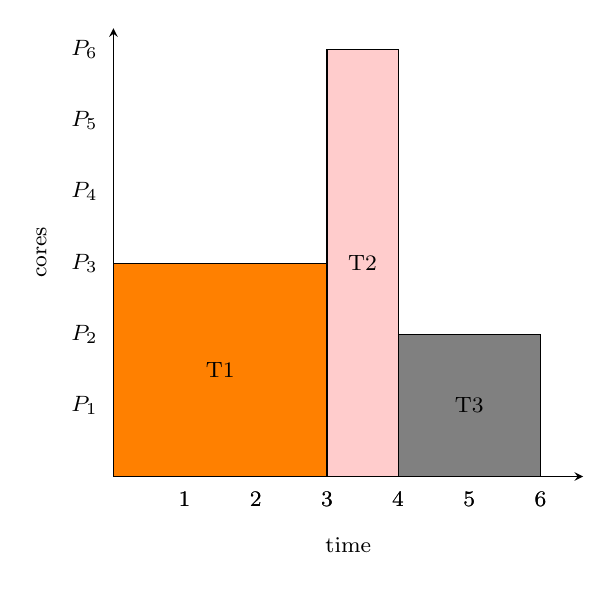
\begin{tikzpicture}\begin{axis}
[ font=\footnotesize,
  ytick style={draw=none},
  xtick style={draw=none},
  unit vector ratio*=1 1 1,
  axis lines = middle,
  enlarge x limits = {value=.1,upper},
  enlarge y limits = {value=.05,upper},
  ylabel={cores},
  xlabel={time},
  ylabel near ticks,
  xlabel near ticks,
  const plot,
  stack plots=false,
  area style,
  ytick={1,...,6},
  yticklabels={},  
  xtick={1,...,6},
  extra y ticks={1,2,3,4,5,6},
  extra x ticks={1,2,3,4,5,6},
  extra y tick style={yticklabel={$P_{\pgfmathprintnumber{\tick}}$}}] 
\addplot[fill=orange] coordinates {(0,0) (0,3) (3,3) (3,0)} node at (current path bounding box.center) {T1}; 
\addplot[fill=red!20] coordinates {(3,0) (3,6) (4,6) (4,0)} node at (current path bounding box.center) {T2}; 
\addplot[fill=gray] coordinates {(4,0) (4,2) (6,2) (6,0)} node at (current path bounding box.center) {T3};  
\end{axis}\end{tikzpicture}

Under our model, a fair baseline would be a scheduler capable
of reducing file transfers while keeping the First-Come-First-Serve
principle. This scheduler is Earliest-Finish-Time (or EFT).
It's an enhanced version of FCFS which chooses to schedule a job
on the node with the earliest available finish time, thus considering
the time to load the file, and consequently choosing nodes where a file will
be re-used. 
\todo[inline]{Max: Say that EFT with bf consider completion time as well.}

%~ For each job in queue
	%~ For each node in Nodeset
		%~ compter le EAT comme pour fcfs
		%~ compute transfer_k corresponding to the time at which F(J) is available mettre un comment sur le calcul (il peut etre deja la ou en partie) (pour calculer la durre ce sera transfer - tk)
		%~ choose node with smallest transfer_k (or tk')
		
		
		

\begin{algorithm}[htbp]
	\caption{Earliest-Finish-Time with conservative backfilling (EFT-BF) (Draft)}\label{algo.fcfsbf}
	\begin{algorithmic}[1]
		\State Job $J_i$ needs to be scheduled. Current time is $current\_time$.
		\ForEach{$\Node{k} \in \nodeset$}
			\State Find $t_k$, the time at which $\core(J_i)$ cores are available
			\If {$\file(J_i) \in \file(\Node{k})$}
				\State $transfer\_time_k \gets 0$
			\Else
				\State $transfer\_time_k \gets \frac{\memory(\file(J_i))}{\bandwidth}$ 
			\EndIf \Comment{Comment représenter le fait d'attendre un chargement par une autre tâche, ce qui peut donner un temps d'attente inférieur au temps de chargement de la donnée?}
		\EndFor
		\State Find $\Node{best\_node} \in \nodeset$ such that $t_{best\_node} + transfer\_time_{best\_node} $ is minimal
		\If{$t_ {best\_node}= current\_time$}
			\State Return $J_i$ scheduled on $\Node{best\_node}$ at time $current\_time$
		\Else
			\ForEach{$\Node{l} \in \nodeset$}
				\State Find $shadow_l$, the time at which less than $\core(J_i)$ cores will be available
				\If {$\file(J_i) \in \file(\Node{l})$}
					\State $transfer\_time_l \gets 0$
				\Else
					\State $transfer\_time_l \gets \frac{\memory(\file(J_i))}{\bandwidth}$
				\EndIf
			\EndFor
			\State Find $\Node{l} \in \nodeset$ such that $transfer\_time_{l} $ is minimal
			\If{$current\_time + \walltime(J_i) \leq shadow_l$}
				\State Return $J_i$ scheduled on $\Node{l}$ at time $current\_time$
			\EndIf
			\State Return $J_i$ scheduled on $\Node{best\_node}$ at time $t_{best\_node}$
		\EndIf
	\end{algorithmic}
\end{algorithm}


Coupled with it, we add the conservative backfilling strategy mentioned earlier:

\subsection{A locality-focused algorithm: SCORE\todo{Max: Or another name}}

The previous strategies are focusing on starting as soon as possible (FCFS)
of finishing as soon as possible a job (EFT).
Those are good methods to avoid starvation of a node and reduce queue times.
However, they are ignoring the effect multiplying the number of copy of a file
over multiple nodes. Indeed, selecting different nodes for jobs using a common
file will increase file loads in order to minimize immediate queue times.
Our strategy (called SCORE) aims at favoring locality in order to reduce
queue times in the long run by reusing the same files. 

The main principle of our algorithm detailed in Algorithm~\ref{algo.score} 
is to find a balance between the earliest available time and data locality,
with a tiebreak on data eviction. A score composed of the earliest available 
time, the time to load or wait for the files to be available and the cost of 
reloading evicted files is computed for each node. The job is then scheduled
on the node with the lowest score.

\begin{algorithm}[htbp]\caption{SCORE (Draft)}\label{algo.score}\begin{algorithmic}[1]
	\State Job $J_i$ needs to be scheduled. Current time is $current\_time$.
	\State $B\_multiplier \gets 500$
	\ForEach {$\Node{k} \in \nodeset$}
		\State Find $t_k$, the time at which $\core(J_i)$ cores are available
		\State $B \gets$ the time to load $\file(J_i)$ on $\Node{k}$ at time $t_k$ \Comment{Or time waiting for the file to be loaded by another job.}
		\State Let $\mathit{sub\_J}$ be the subset of jobs that ends right before time $t_k$ on $\Node{k}$
		\State $C \gets (\memory(\file(\mathit{sub\_J})) \times \frac{\core(J_i)}{\core(\Node{k})})/\bandwidth$
		\State $score_{\Node{k}} \gets t_k + B\_multiplier \times B + C$
	\EndFor
	\State Schedule $J_i$ on the node with the smallest score. Tiebreak with lowest node's id.
\end{algorithmic}\end{algorithm}

\begin{algorithm}[htbp]
\caption{EFT-SCORE MIX (Draft)}
\begin{algorithmic}[1]
	\State Job $J_i$ needs to be scheduled. Current time is $current\_time$
	\State $occupation\_threshold \gets 80$ 
	\State $occupation \gets$ the percentage of nodes running at least one job at time $current\_time$
	\If{$occupation < occupation\_threshold$}
		\State $EFT(\jobset,\nodeset)$
	\Else
		\State $SCORE(\jobset,\nodeset)$
	\EndIf
\end{algorithmic}
\end{algorithm}

\begin{algorithm}[htbp]
\caption{OPPORTUNISTIC-SCORE MIX (Draft)}
\begin{algorithmic}[1]
	\State Job $J_i$ needs to be scheduled. Current time is $current\_time$
	\State $B\_multiplier \gets 500$
	\State $C\_multiplier \gets 1$
	\ForEach {$\Node{k} \in \nodeset$}
		\State Find $t_k$, the time at which $\core(J_i)$ cores are available
		\If{$t_k = current~time$}
			\State $B\_multiplier \gets 1$
			\State $C\_multiplier \gets 0$
		\EndIf
		\State $B \gets$ the time to load $\file(J_i)$ on $\Node{k}$ at time $t_k$
		\State Let $\mathit{sub\_J}$ be the subset of jobs that ends right before time $A$ on $\Node{k}$
		\State $C \gets (\memory(\file(\mathit{sub\_J})) \times \frac{\core(J_i)}{\core(\Node{k})})/\bandwidth$
		\State $score_{\Node{k}} \gets t_k + B\_multiplier \times B + C\_multiplier \times C$
	\EndFor
	\State Schedule $J_i$ on the node with the smallest score. Tiebreak with lowest node's id.
\end{algorithmic}
\end{algorithm}

\begin{algorithm}[htbp]
\caption{Score with conservative backfilling (SCORE-BF) (Draft)}
\begin{algorithmic}[1]
	\State Job $J_i$ needs to be scheduled. Current time is $current\_time$.
	\State $B\_multiplier \gets 500$
	\ForEach {$\Node{k} \in \nodeset$}
		\State Find $t_k$, the time at which $\core(J_i)$ cores are available
		\State $B \gets$ the time to load $\file(J_i)$ on $\Node{k}$ at time $t_k$ \Comment{Or time waiting for the file to be loaded by another job.}
		\State Let $\mathit{sub\_J}$ be the subset of jobs that ends right before time $t_k$ on $\Node{k}$
		\State $C \gets (\memory(\file(\mathit{sub\_J})) \times \frac{\core(J_i)}{\core(\Node{k})})/\bandwidth$
		\State $score_{\Node{k}} \gets t_k + B\_multiplier \times B + C$
	\EndFor
	\ForEach{$\Node{l} \in \nodeset$}
		\State Find $shadow_l$, the time at which less than $\core(J_i)$ cores will be available
			\If{$current\_time + \walltime(J_i) \leq shadow_l$}
				\State $B \gets$ the time to load $\file(J_i)$ on $\Node{l}$ at time $current\_time$
				\State Let $\mathit{sub\_J}$ be the subset of jobs that ends right before time $current\_time$ on $\Node{l}$
				\State $C \gets (\memory(\file(\mathit{sub\_J})) \times \frac{\core(J_i)}{\core(\Node{k})})/\bandwidth$
				\If{$score_{\Node{l}} > current\_time + B\_multiplier \times B + C$}
					\State $score_{\Node{l}} \gets current\_time + B\_multiplier \times B + C$
				\EndIf
			\EndIf
	\EndFor
	\State Schedule $J_i$ on the node with the smallest score. Tiebreak with lowest node's id.	
	
	%~ \State Job $J_i$ needs to be scheduled. Current time is $current\_time$
	%~ \State $B\_multiplier \gets 500$
	%~ \State $C\_multiplier \gets 1$
%~ \ForEach {$J_i \in \jobset$}
	%~ \ForEach {$\Node{k} \in \nodeset$}
		%~ \State $A \gets$ the earliest available time to compute $J_i$ on $\Node{k}$
		%~ \State $B \gets$ the time to load $\file(J_i)$ on $\Node{k}$ at time $A$
		%~ \State Let $\mathit{sub\_J}$ be the subset of jobs that ends right before time $A$ on $\Node{k}$
		%~ \State $C \gets (\file(\mathit{sub\_J}) \times \frac{\core(J_i)}{\core(\Node{k})})/\bandwidth$
		%~ \State $score_{\Node{k}} \gets A + B\_multiplier \times B + C\_multiplier \times C$
		%~ \If {$\Node{k}$ has a hole and $j_i$ can use it}
			%~ \State $A \gets current~time$
			%~ \State $B \gets$ the time to load $\file(J_i)$ on $\Node{k}$ at time $A$
			%~ \State Let $\mathit{sub\_J}$ be the subset of jobs that ends right before time $A$ on $\Node{k}$
			%~ \State $C \gets (\file(\mathit{sub\_J}) \times \frac{\core(J_i)}{\core(\Node{k})})/\bandwidth$
			%~ \State $score_{\mathit{Cores\_Hole}(\Node{k})} \gets A + B\_multiplier \times B + C\_multiplier \times C$
		%~ \EndIf
	%~ \EndFor
	%~ \State Schedule $J_i$ on the node or hole with the best score. Schedule on the node with the lowest index in case of a tie.
	%~ \If {$Backfill\_mode = 1$ OR $Backfill\_mode = 2$}
		%~ \State Minimize hole creation when affecting cores to $j_i$
		%~ \If {$Backfill\_mode = 1$}
			%~ \State Schedule $j_i$ on the cores with the biggest next start time
		%~ \Else
			%~ \State Schedule $j_i$ on the cores with the smallest next start time
		%~ \EndIf
	%~ \EndIf
%~ \EndFor
\end{algorithmic}
\end{algorithm}

\section{Working with information from a real workload and cluster\todo[inline]{Max: Another name for this section?}}\label{sec.working}
Actual workloads at HPC resources shared by a great number of users with diverse needs can contain structures
that are non-trivial to replicate in a fully artificial simulated job pattern. We believe that this is especially
true for data-dependent patterns, where a project might launch a burst of jobs using the same file just a few thousand
core hours in length, then be quiet for a long time processing the results, and then launch another such burst.

On the other hand, it would be disruptive to expose a real user community to a wide variety of experimental scheduling strategies.

For this reason, we used logs of historical submitted jobs, in terms of their exact submission time, size, stated runtime, and actual runtime.
Since explicit data dependencies are not encoded in SLURM job specifications, we created an artificial pattern for this. 
\todo[inline]{Carl: Max, please elaborate. Max: Okay, I added a paragraph.}
Each job is carrying an input file.
Let's consider two jobs from the logs of historical submitted jobs: $J_i$ and $J_j$.
They will be attributed a common input file if they match all the following requirements:
\begin{enumerate}
	\item $\core(J_i) = \core(J_j)$ i.e they are requiring the same amount of cores.
	\item $J_i$ and $J_j$ were submitted by the same user.
	\item $J_i$ and $J_j$ were submitted in a 800 seconds timeframe.
\end{enumerate}
Otherwise we consider that $J_i$ and $J_j$ are using distinct input files.

\todo[inline]{Elisabeth: I think we should say Rackham so that readers can checkout the hardware, but perhaps it should be fully blind as a starting point.}
The resource consists of 486 nodes with 20 cores each, with most of them having 128GB of RAM, with some 256GB and 512GB nodes. \todo[inline]{Max: I thought it was 1024 GB nodes for the biggest size?}

\todo[inline]{Max: I added a paragraph on why all nodes are the same size in our case:}
Having $L$ different nodes sizes raises a new constraint. The model would have
$L$ subsets of nodes, each possibly containing a different number of nodes.
An input file can be too large to be computed on one or multiple of those subsets.
Thus, in addition to the scheduling problem, a load balancing problem arises.
Indeed, the scheduler need to be able to manage each subset of nodes as an independant 
resource that need to avoid starvation while also not being saturated in case of a large
batch of jobs that could be submitted at once and that could only be computed on this node's size.
Consequently, to focus on the issue of data-locality, we use a set of 486 nodes of size 
128 GB and the size of an input file is a multiple of 6.4.
In other words, for each $\file(i) \in \fileset$, $\memory(\file(i)) = 6.4 \times n$ with 
$1 \leq n \leq 20$.

The utilization levels are typically high ($>90\%$), but
not fully consistently so. The vast majority of jobs on this resources are single node jobs, even sometimes single core jobs. Run times
could extent to up to 10 days, while some jobs only last a few minutes. We do not claim that this is an ideal job submission strategy,
but rather it is an empirical observation of an actual user community including, but not exclusively consisting of, many subfields of the life sciences with highly data-dependent workflows.

\section{Performance evaluation and analysis}\label{sec.evaluations}

We present below the results of experimental evaluations conducted 
on X\todo[inline]{Max: To update once all experiments are complete} days
from a real workload history.

\subsection{Settings\todo[inline]{Maybe this section should be merged with the one above?}}

All strategies as well as the two baselines have been implemented on
a simulator that we developed. Each application scenario is a day on the log's history of
the workload.
The way we collect jobs from the log's history is represented in Figure~\ref{fig.workload}.

\begin{figure*}[tb]
\definecolor{blue}{rgb}{0.38, 0.51, 0.71} %glaucous, 97,130,181, #6182B5
\definecolor{darkblue}{RGB}{17, 42, 60} % 112A3C
\definecolor{red}{RGB}{175, 49, 39} % AF3127
\definecolor{otherred}{RGB}{171,78,78}
\definecolor{orange}{RGB}{237, 126, 75} 
\definecolor{green}{RGB}{104, 174, 89} 
\definecolor{palegreen}{RGB}{197, 184, 104} 
\definecolor{yellow}{RGB}{250, 199, 70} % FAC764
\definecolor{brokenwhite}{RGB}{218, 192, 166} % DAC0A6
\definecolor{brokengrey}{rgb}{0.77, 0.76, 0.82} % {196,194,209}, C4C2D1
\centering\scalebox{1}{
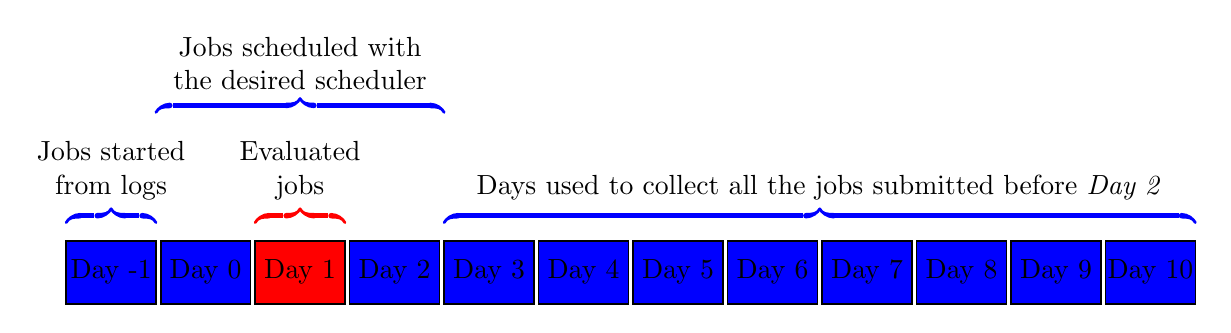
\begin{tikzpicture}[semithick, > = {Stealth[scale=1.25]}, shorten > = 1pt,]
    \def\x{1}\def\y{1}
    \draw[color=black, fill=blue] (0*\x+0.03, 0.7) rectangle (1.2*1*\x-0.03, -0.1) node[midway] {Day -1}; 
    \draw[color=black, fill=blue] (1.2*1*\x+0.03, 0.7) rectangle (1.2*2*\x-0.03, -0.1) node[midway] {Day 0}; 
    \draw[color=black, fill=red] (1.2*2*\x+0.03, 0.7) rectangle (1.2*3*\x-0.03, -0.1) node[midway] {Day 1}; 
    \draw[color=black, fill=blue] (1.2*3*\x+0.03, 0.7) rectangle (1.2*4*\x-0.03, -0.1) node[midway] {Day 2}; 
    \draw[color=black, fill=blue] (1.2*4*\x+0.03, 0.7) rectangle (1.2*5*\x-0.03, -0.1) node[midway] {Day 3}; 
    \draw[color=black, fill=blue] (1.2*5*\x+0.03, 0.7) rectangle (1.2*6*\x-0.03, -0.1) node[midway] {Day 4}; 
    \draw[color=black, fill=blue] (1.2*6*\x+0.03, 0.7) rectangle (1.2*7*\x-0.03, -0.1) node[midway] {Day 5}; 
    \draw[color=black, fill=blue] (1.2*7*\x+0.03, 0.7) rectangle (1.2*8*\x-0.03, -0.1) node[midway] {Day 6}; 
    \draw[color=black, fill=blue] (1.2*8*\x+0.03, 0.7) rectangle (1.2*9*\x-0.03, -0.1) node[midway] {Day 7}; 
    \draw[color=black, fill=blue] (1.2*9*\x+0.03, 0.7) rectangle (1.2*10*\x-0.03, -0.1) node[midway] {Day 8}; 
    \draw[color=black, fill=blue] (1.2*10*\x+0.03, 0.7) rectangle (1.2*11*\x-0.03, -0.1) node[midway] {Day 9}; 
    \draw[color=black, fill=blue] (1.2*11*\x+0.03, 0.7) rectangle (1.2*12*\x-0.03, -0.1) node[midway] {Day 10}; 
    
    %~ \draw (4*\x,2*\y) node[right]{\it \small data in memory};
    \draw [pen colour={blue},decorate,line width=2pt,decoration = {calligraphic brace,raise=-2pt,amplitude=5pt}] (0*\x+0.03, 1) -- node[pos=0.5,above=2pt,black,align=center]{Jobs started\\from logs} (1.2*1*\x-0.03, 1);
    \draw [pen colour={blue},decorate,line width=2pt,decoration = {calligraphic brace,raise=-2pt,amplitude=5pt,mirror}] (1.2*4*\x+0.03, 2.4) -- node[pos=0.5,above=2pt,black,align=center]{Jobs scheduled with\\the desired scheduler} (1.2*1*\x-0.03, 2.4);
    \draw [pen colour={blue},decorate,line width=2pt,decoration = {calligraphic brace,raise=-2pt,amplitude=5pt}] (1.2*4*\x+0.03, 1) -- node[pos=0.5,above=2pt,black,align=center]{Days used to collect all the jobs submitted before \textit{Day 2}} (1.2*12*\x-0.03, 1);
    \draw [pen colour={red},decorate,line width=2pt,decoration = {calligraphic brace,raise=-2pt,amplitude=5pt}] (1.2*2*\x+0.03, 1) -- node[pos=0.5,above=2pt,black,align=center]{Evaluated\\jobs} (1.2*3*\x-0.03, 1);
  \end{tikzpicture}
}
\caption{}\label{fig.workload}
\label{fig.ex}
\end{figure*}

In the log's history, each time a jobs finished, it's information
are noted in a file corresponding to the day at which the day finished.
This information contains the node that was attributed, the real job's duration, the walltime, 
the number of cores required, the user that submitted the job, the submission time, 
the start and end time.
Thus, in order to get all the jobs that were submitted on \textit{Day 1}, we will
look into the logs of days 1 to 10. Indded, most jobs do not last for more than 10 days,
thus we should cover the vast majority of jobs that were actually submitted on 
\textit{Day 1}. 
Jobs of \textit{Day 1} are preceded and succeded with jobs from \textit{Day 0}
and \textit{Day 2} in order to place \textit{Day 1} in its "real environment",
i.e. in the situation in which it was on the real cluster, with jobs submitted
before and after.
Jobs from \textit{Day -1} are jobs that were submitted before \textit{Day 0}.
We use the information from the log's history to start this jobs on the nodes
were they really were scheduled at the times at which they were started.
This allows us to exactly replaate the state of thecluster on this day before starting
to schedule jobs from \textit{Day 0} with our choosen scheduler.

\subsection{Results on an under-used cluster}

Figure~\ref{07_16_cluster_usage} shows us a visual representation of 
our cluster's usage over time. The solid black dotted line is the total
number of cores available.
\todo[inline]{Max: Change the label once we know which one is the first shown figure of this type}
The solid blue line shows the number of cores occupied by running jobs.
The dashed blue line shows the additional number of cores that would be needed
to run all the jobs in the queue at a given time (this would thus be the number
of used cores if all the jobs where running in parallel).
The red lines show the jobs in both categories that have their submission
time within our evaluation window, in other words they are sub-parts of the blue line
that we evaluate.

\begin{figure}[H]\centering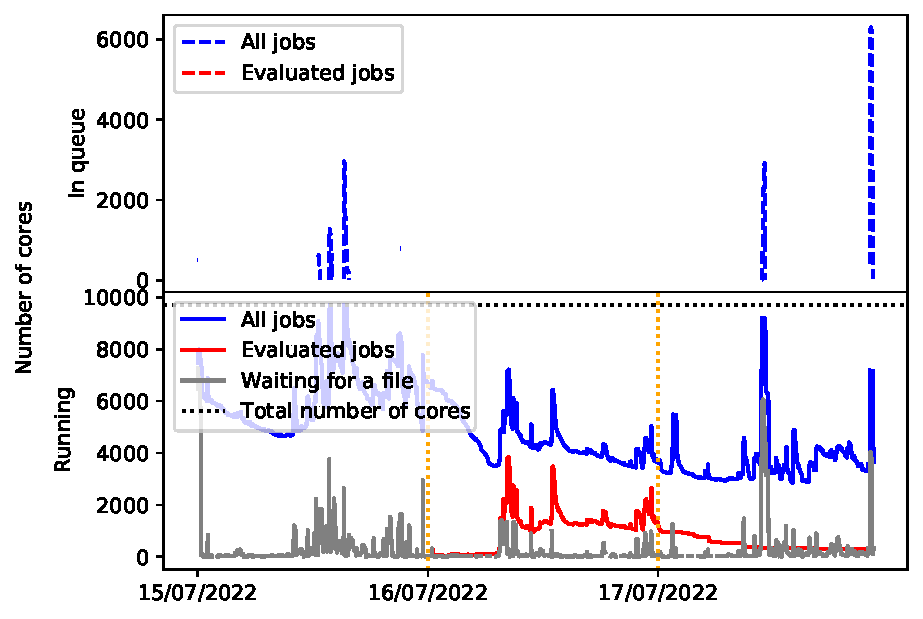
\includegraphics[width=1\linewidth]{../MBSS/plot/Cluster_usage/2022-07-16->2022-07-16_V10000_Fcfs_Used_nodes_Reduced_450_128_32_256_4_1024_core_by_core.pdf}\caption{Visualization of the utilization rate of the cluster on the workload of July the 16th with FCFS.\todo[inline]{Elisabeth: I guess you will explain the graph somewhere, but right now, evaluated is ambiguous for me. When I read it I think finished jobs, but I assume it means jobs that will be in the schedule(?) Why are the two dashed ones flatlined? I assume it is becasue the queue is ``wider'' than all cores(?) Nice that the window is more visible. }}\end{figure}
\begin{figure}[H]\centering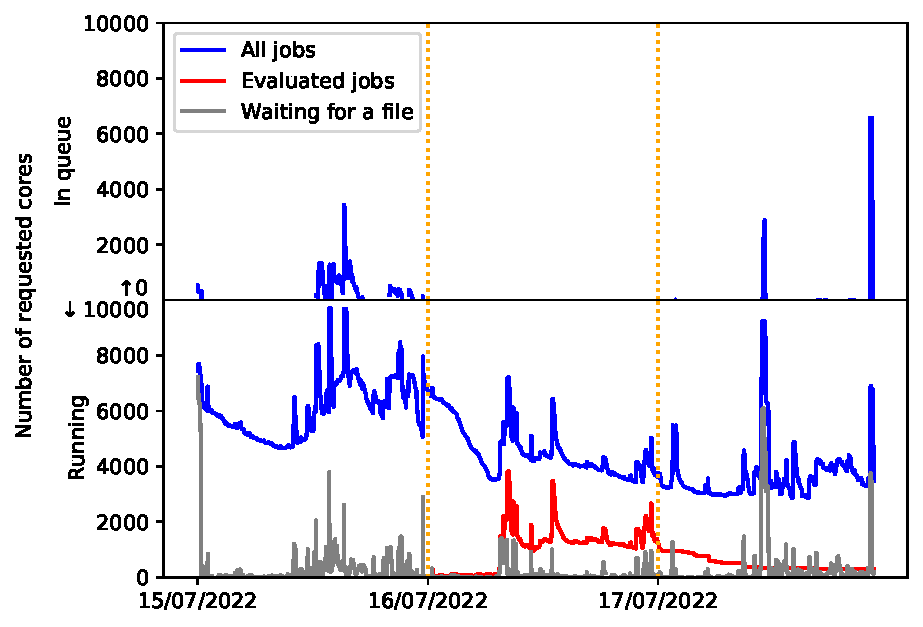
\includegraphics[width=1\linewidth]{../MBSS/plot/Cluster_usage/2022-07-16->2022-07-16_V10000_Fcfs_with_a_score_mixed_strategy_x500_x1_x0_x0_Used_nodes_Reduced_450_128_32_256_4_1024_core_by_core.pdf}\caption{Cluster's usage with EFT-SCORE MIX - Workload of July 16 - Not saturated}\end{figure}
\begin{figure}\centering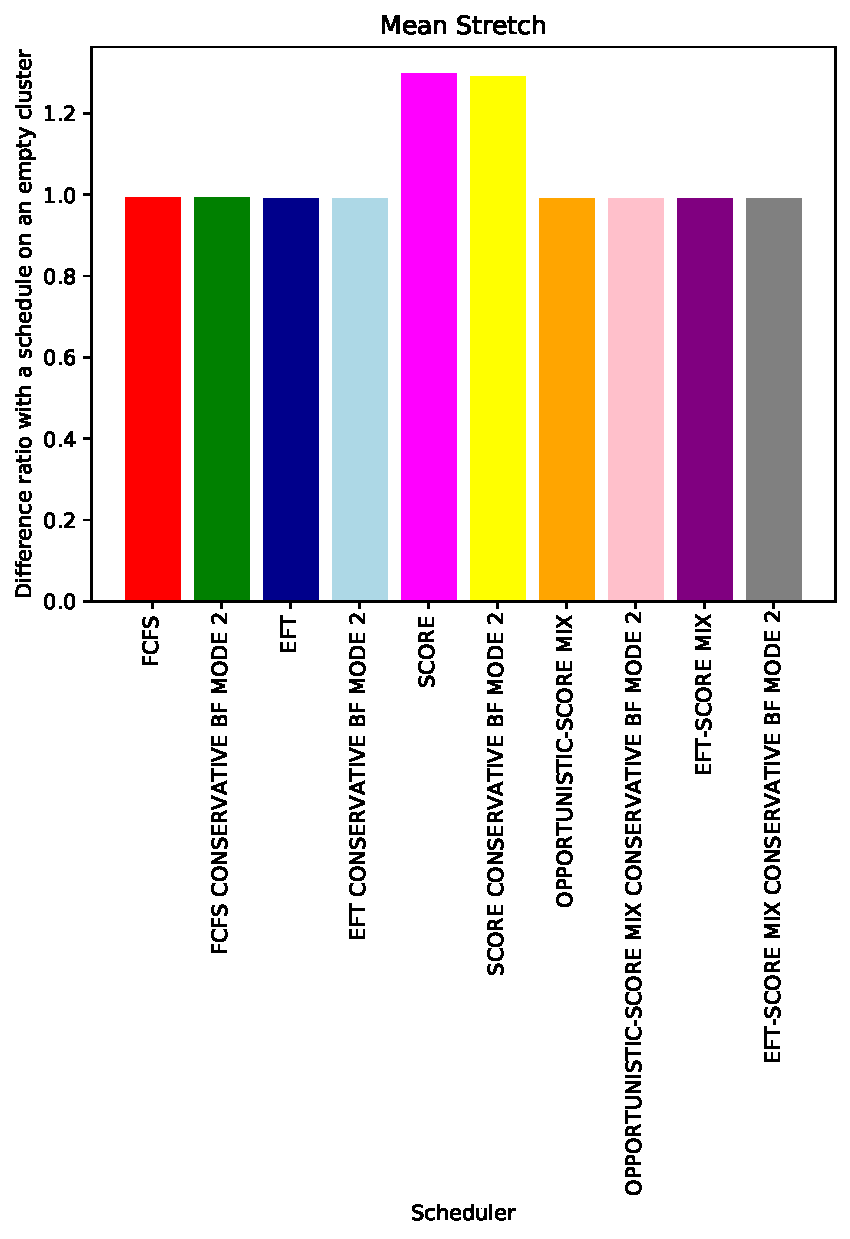
\includegraphics[width=1\linewidth]{../MBSS/plot/Results_FCFS_Score_Backfill_2022-07-16->2022-07-16_V10000_Mean_Stretch_450_128_32_256_4_1024.pdf}\caption{Mean stretch on all jobs - Workload of July 16 \todo[inline]{Elisabeth: How many bars will there be in the end? All of these or less? The names are so long. Could there perhaps be a table that explains the difference between the schedulers and a short acronym for each? This is more a matter of taste.}}\end{figure}
\begin{figure}\centering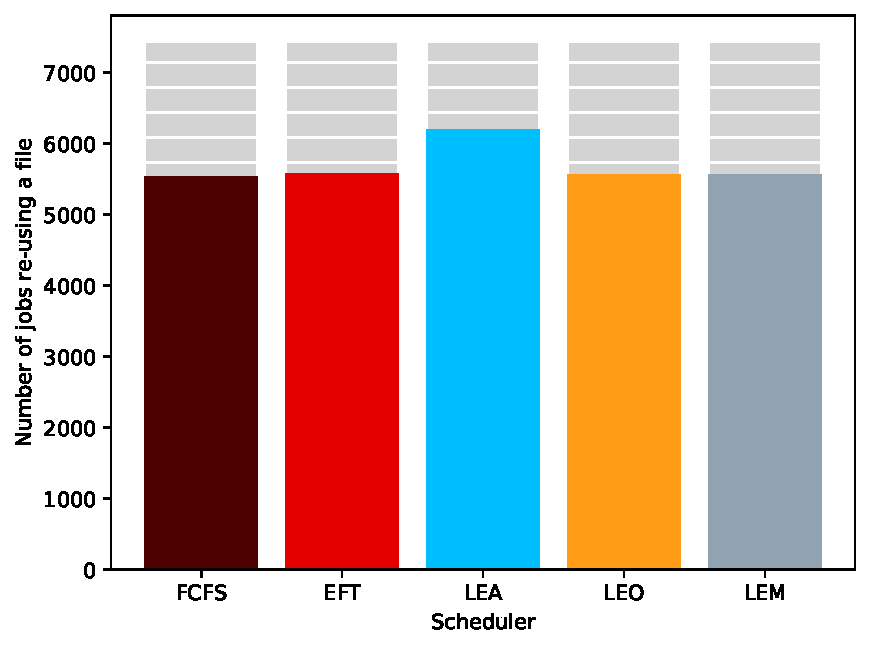
\includegraphics[width=1\linewidth]{../MBSS/plot/Results_FCFS_Score_Backfill_2022-07-16->2022-07-16_V10000_Number_of_data_reuse_450_128_32_256_4_1024.pdf}\caption{Number of evaluated jobs re-using a data - Workload of July 16\todo[inline]{Elisabeth: Could there also be a second part of the bar showing number of jobs not reusing data? Now I think we can't know how large the fraction is. Max: Okay I did it here in gray.}}\end{figure}

\begin{figure}[H]\centering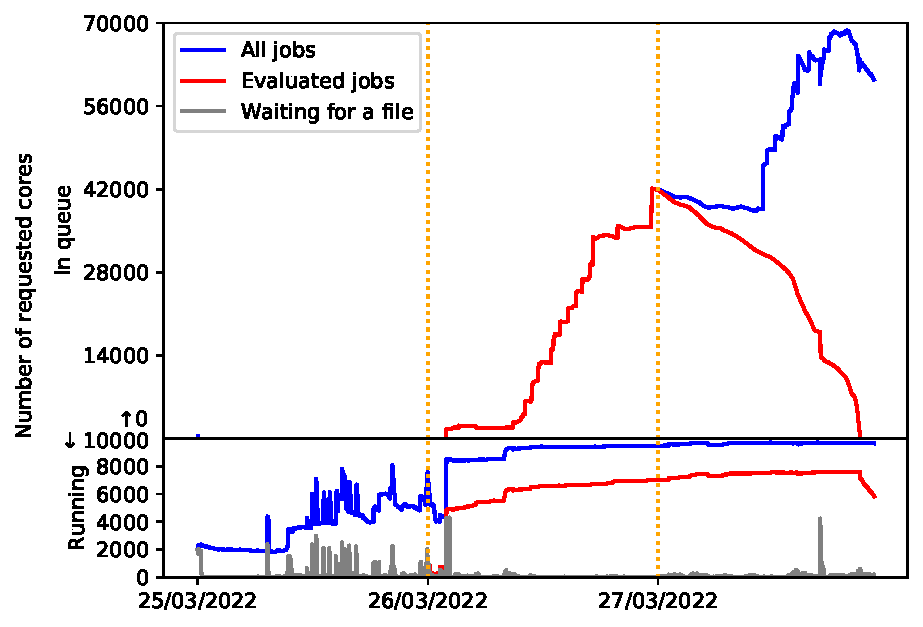
\includegraphics[width=1\linewidth]{../MBSS/plot/Cluster_usage/2022-08-16->2022-08-16_V10000_Fcfs_Used_nodes_Reduced_450_128_32_256_4_1024_core_by_core.pdf}\caption{Visualization of the utilization rate of the cluster on the workload of August the 16th with FCFS.}\end{figure}
%~ \begin{figure}[H]\centering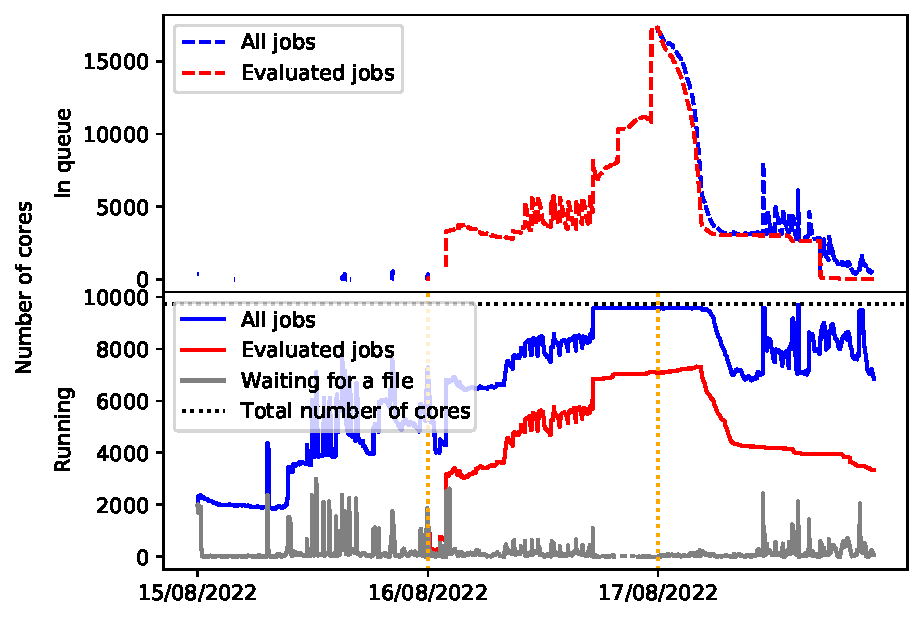
\includegraphics[width=1\linewidth]{../MBSS/plot/Cluster_usage/2022-08-16->2022-08-16_V10000_Fcfs_with_a_score_mixed_strategy_x500_x1_x0_x0_Used_nodes_Reduced_450_128_32_256_4_1024_core_by_core.pdf}\caption{Cluster's usage with EFT-SCORE MIX - Workload of August 16 - Not saturated.}\end{figure}
\begin{figure}\centering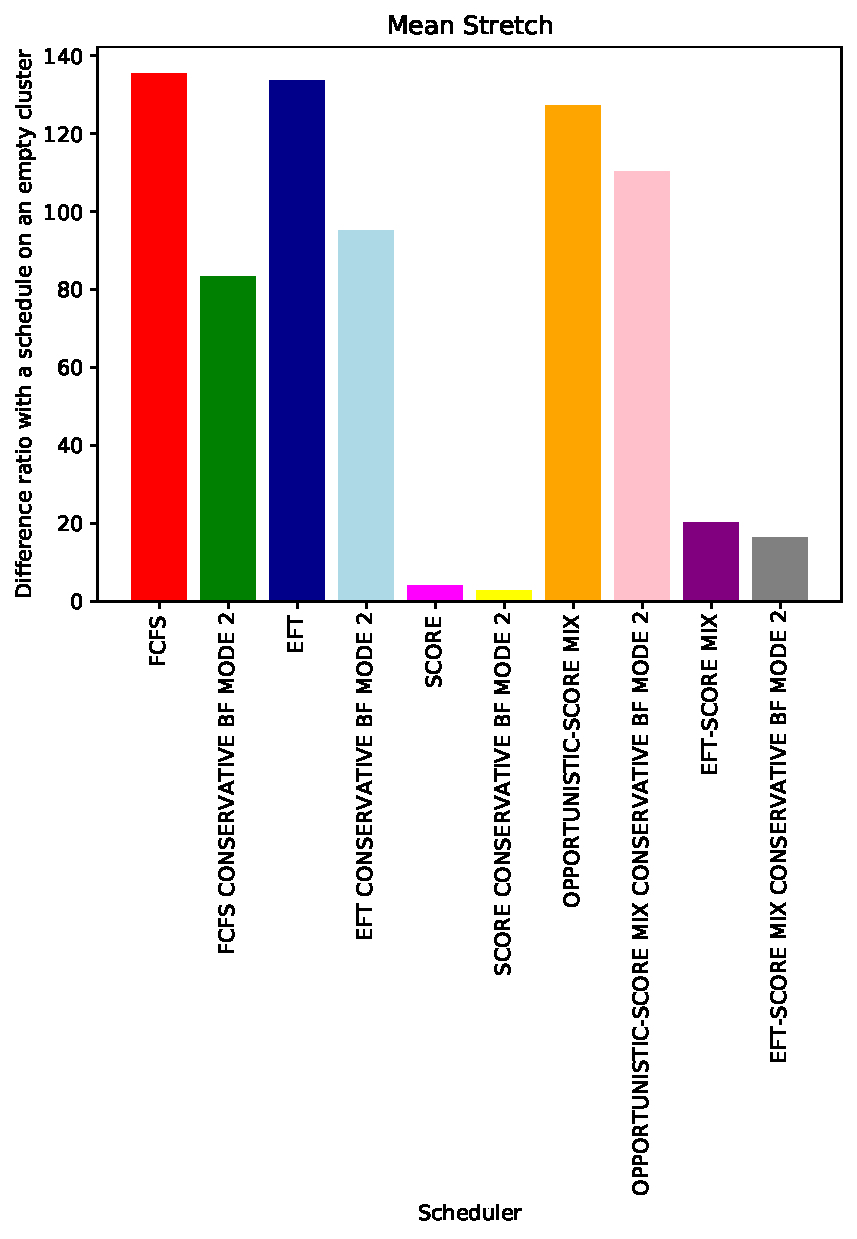
\includegraphics[width=1\linewidth]{../MBSS/plot/Results_FCFS_Score_Backfill_2022-08-16->2022-08-16_V10000_Mean_Stretch_450_128_32_256_4_1024.pdf}\caption{Mean stretch on all jobs - Workload of August 16.}\end{figure}
\begin{figure}\centering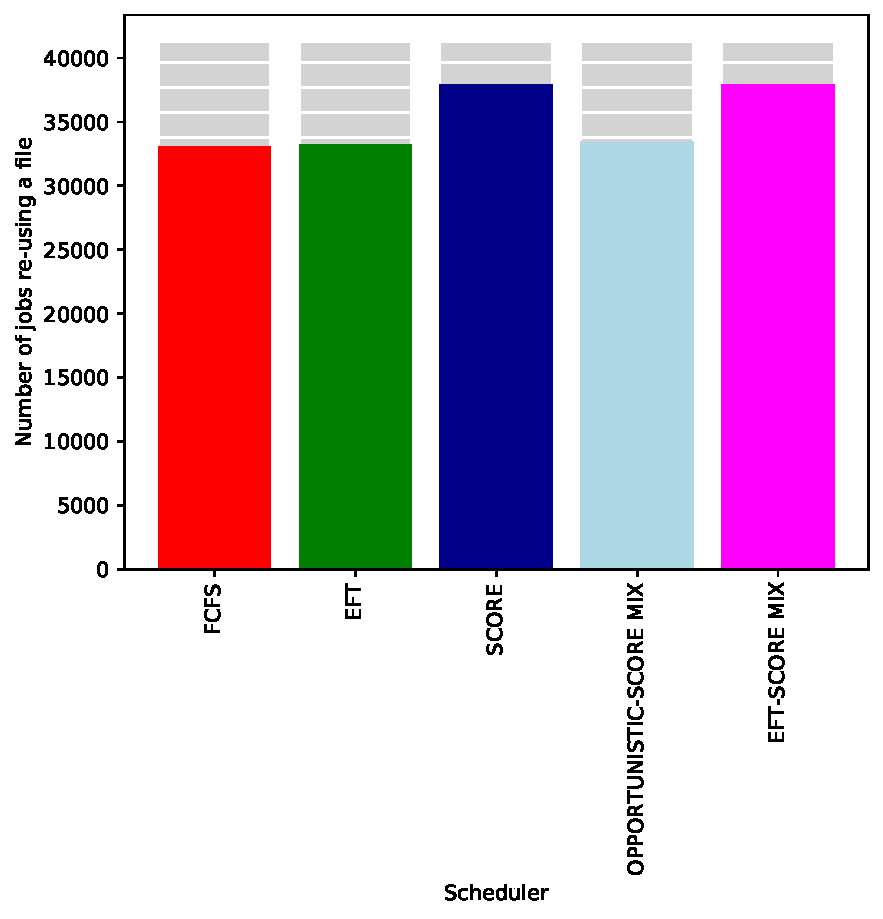
\includegraphics[width=1\linewidth]{../MBSS/plot/Results_FCFS_Score_Backfill_2022-08-16->2022-08-16_V10000_Number_of_data_reuse_450_128_32_256_4_1024.pdf}\caption{Number of evaluated jobs re-using a data - Workload of August 16.}\end{figure}

\begin{figure}\centering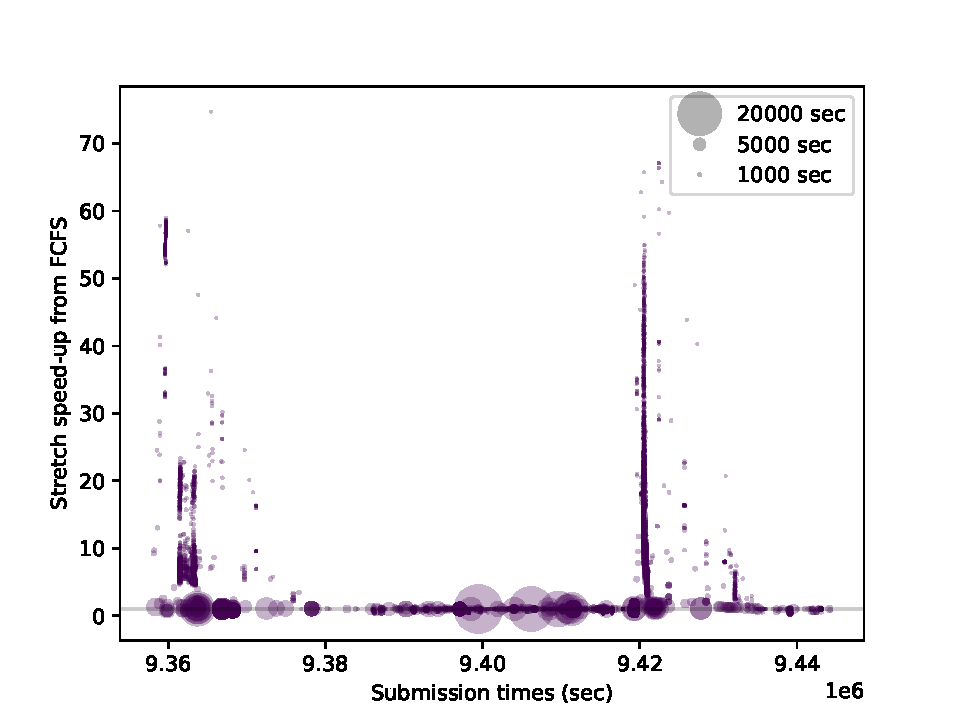
\includegraphics[width=1\linewidth]{../MBSS/plot/Stretch_times/Stretch_times_FCFS_EFT-SCORE-MIX_2022-07-13->2022-07-13_V10000_450_128_32_256_4_1024.pdf}\caption{Stretch speed-up of EFT-SCORE MIX compared to FCFS, job by job on the workload of July 13\todo[inline]{Elisabeth: Also a nice plot. Showing that only when the file loading time is a substantial part of the overall job time is there a large speedup? Max: Yes exactly.}}\end{figure}
\begin{figure}\centering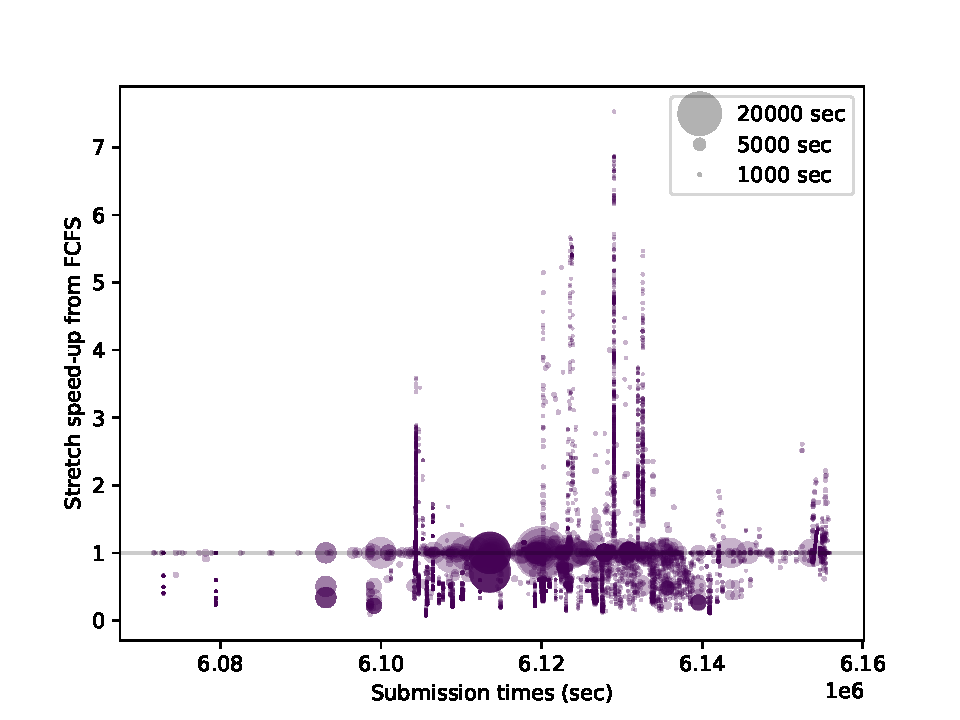
\includegraphics[width=1\linewidth]{../MBSS/plot/Stretch_times/Stretch_times_FCFS_EFT-SCORE-MIX_2022-09-09->2022-09-09_V10000_450_128_32_256_4_1024.pdf}\caption{Stretch speed-up of EFT-SCORE MIX compared to FCFS, job by job on the workload of 09/09.}\end{figure}

\begin{figure}\centering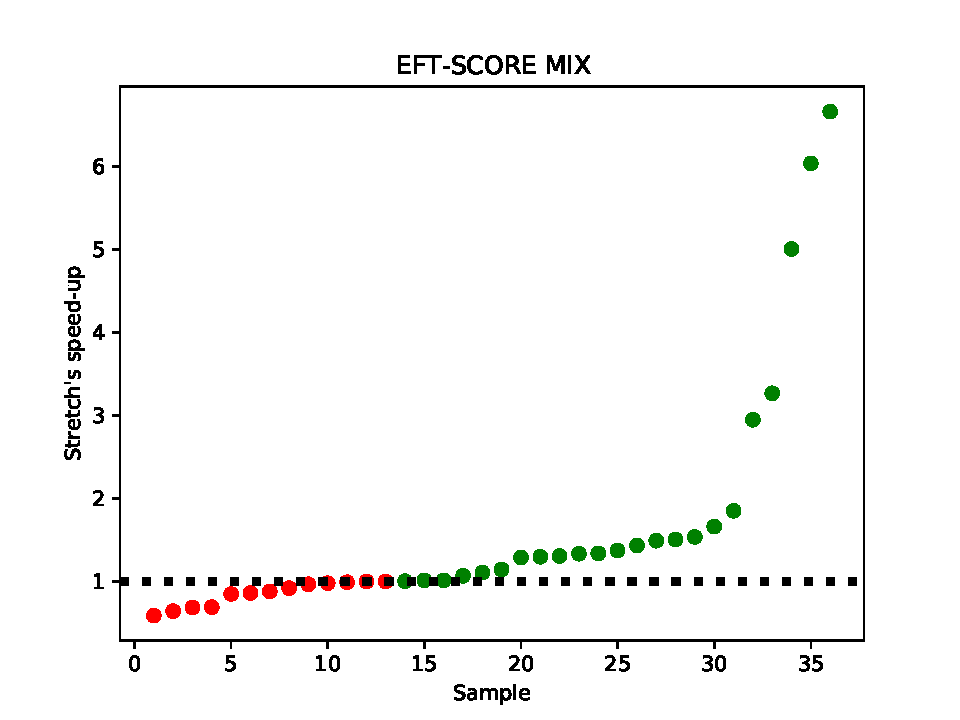
\includegraphics[width=1\linewidth]{../MBSS/plot/Scatter/scatter_mean_stretch_all_workloads_EFT-SCORE-MIX_v1.pdf}\caption{Different color if inferior to 1\todo[inline]{I like these plots, but what is sample?}}\end{figure}
\begin{figure}\centering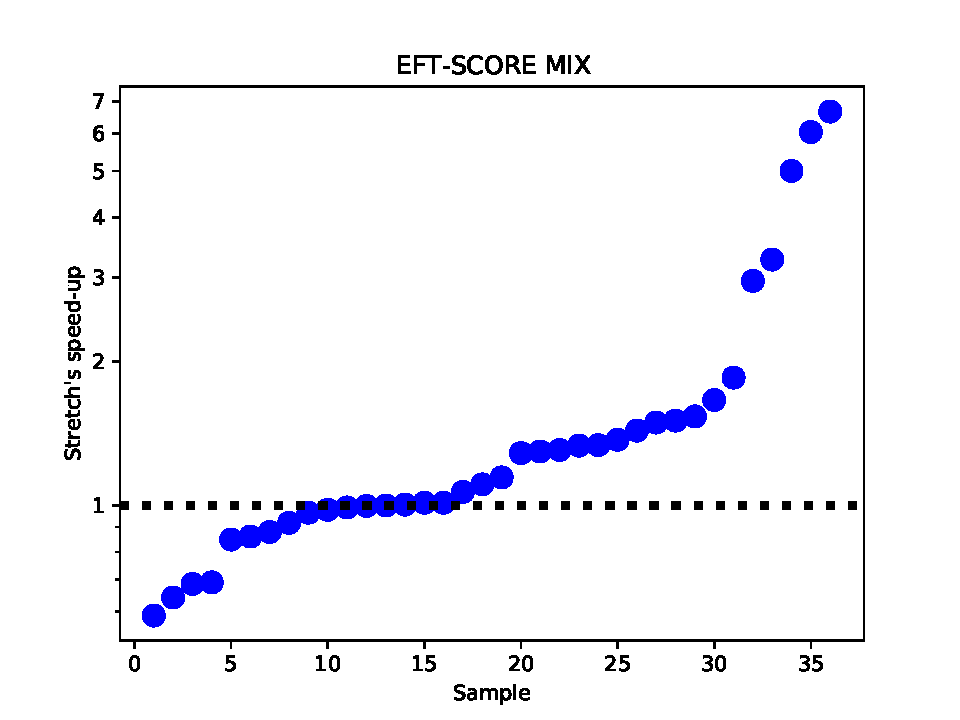
\includegraphics[width=1\linewidth]{../MBSS/plot/Scatter/scatter_mean_stretch_all_workloads_EFT-SCORE-MIX_v3.pdf}\caption{With a log scale.}\end{figure}
\begin{figure}\centering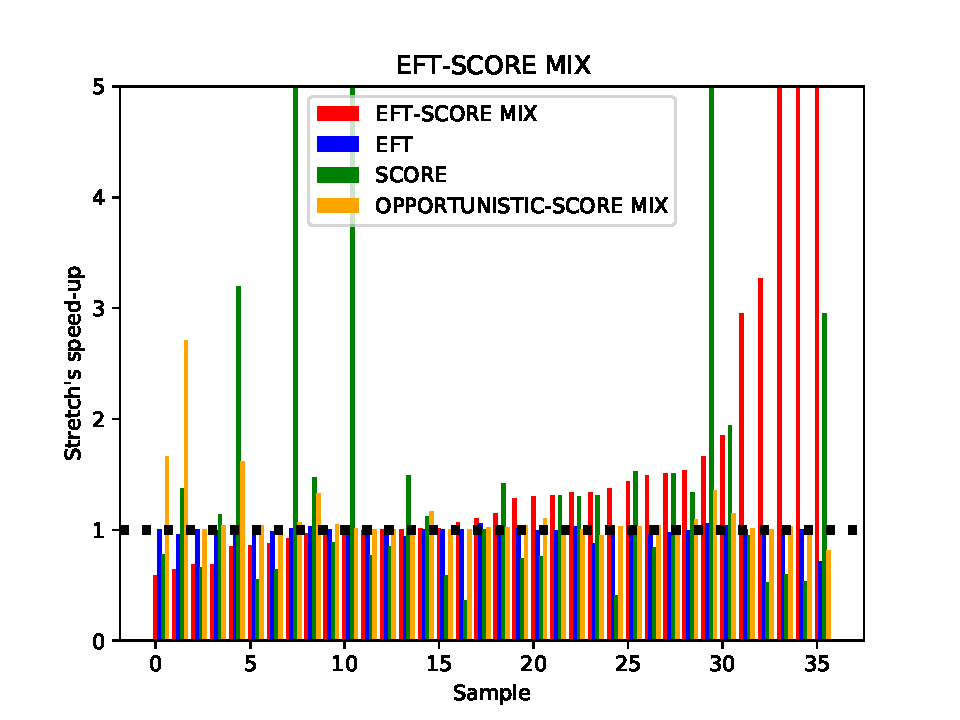
\includegraphics[width=1\linewidth]{../MBSS/plot/Scatter/scatter_mean_stretch_all_workloads_EFT-SCORE-MIX_v2.pdf}\caption{I took the sorted stretches from EFT-SCORE MIX and applied the same order to other schedulers. Barplot instead of points. Added a maximum on the y axis.}\end{figure}

\begin{figure}\centering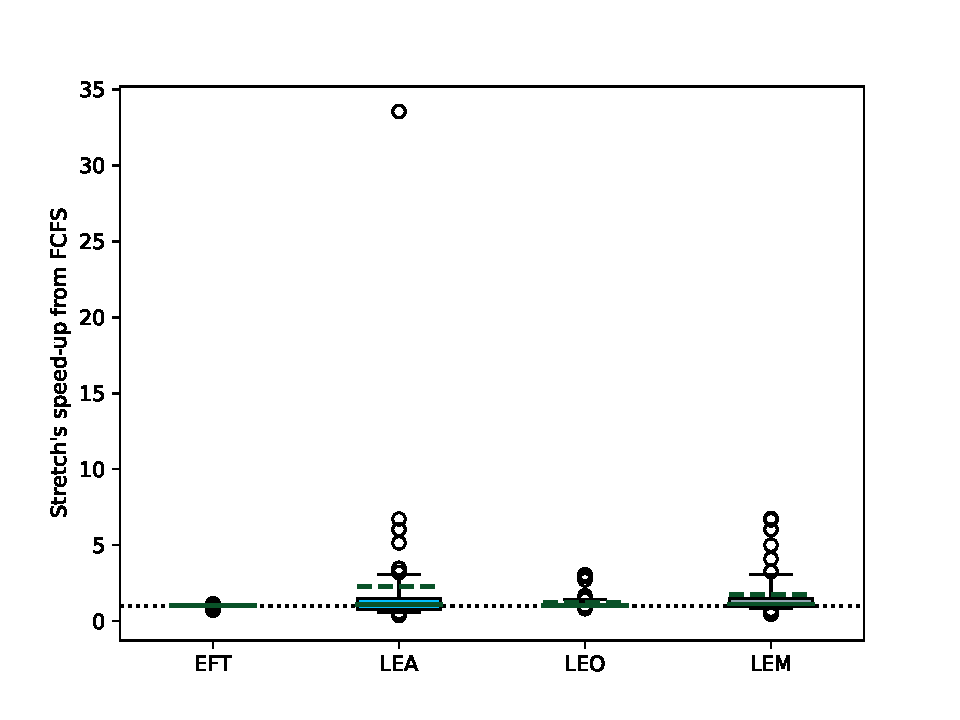
\includegraphics[width=1\linewidth]{../MBSS/plot/Boxplot/box_plot_mean_stretch_all_workloads_full.pdf}\caption{Boxplots full}\end{figure}
\begin{figure}\centering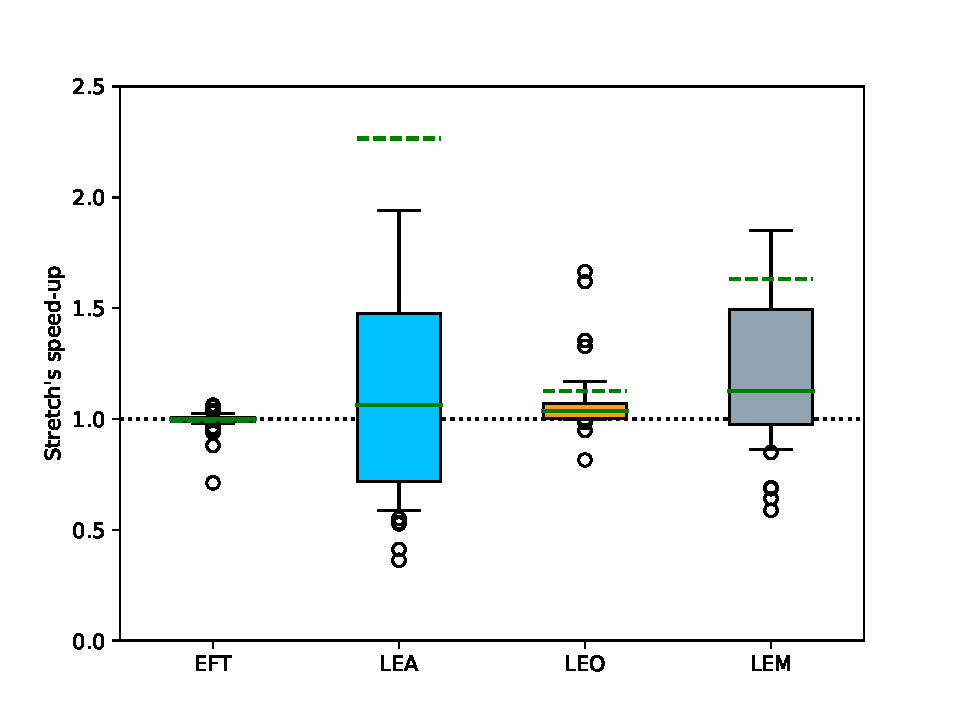
\includegraphics[width=1\linewidth]{../MBSS/plot/Boxplot/box_plot_mean_stretch_all_workloads.pdf}\caption{Boxplots with a max on Y. The whiskers are 25th percentile - 1.5*IQR and 75th percentile + 1.5*IQR with IQR the Interquartile range.}\end{figure}
\begin{figure}\centering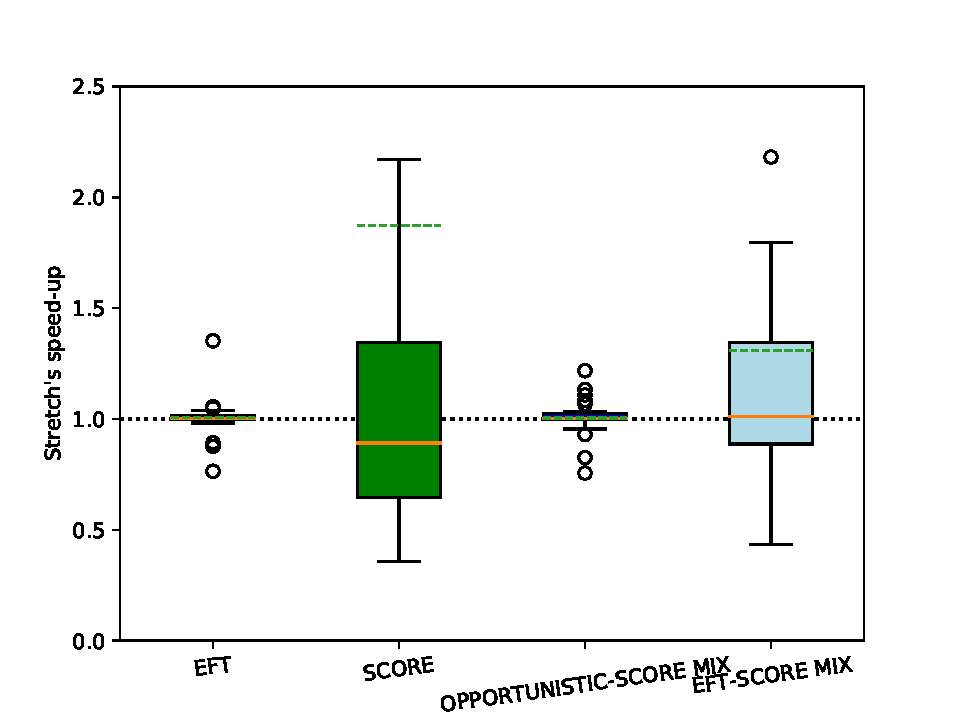
\includegraphics[width=1\linewidth]{../MBSS/plot/Boxplot/box_plot_mean_stretch_all_workloads_bf.pdf}\caption{Boxplots with a max on Y with backfilling}\end{figure}

\begin{figure}\centering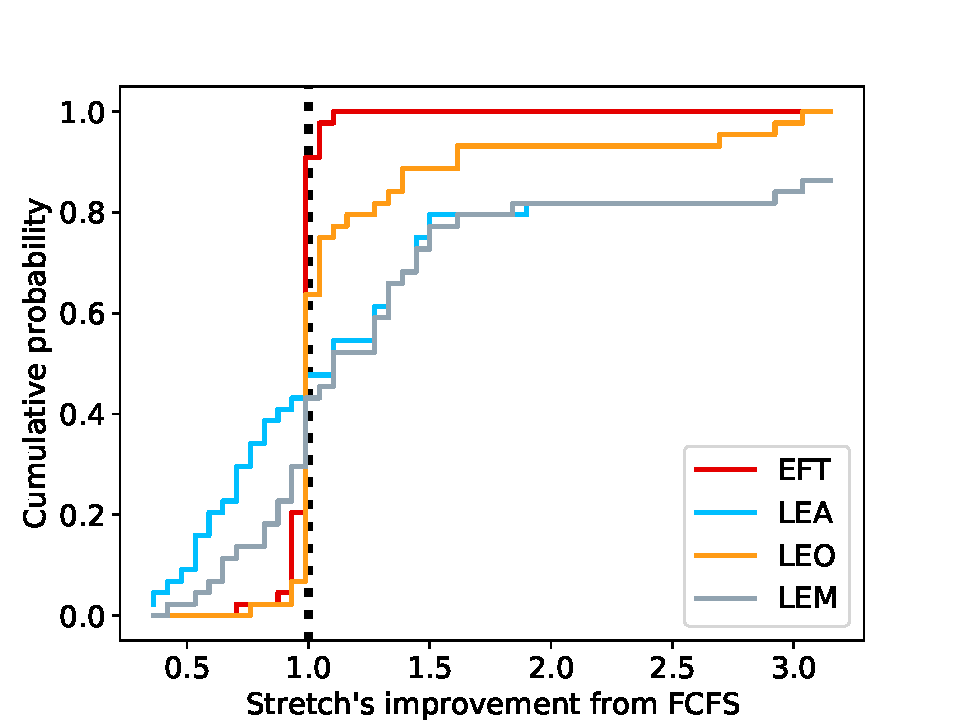
\includegraphics[width=1\linewidth]{../MBSS/plot/ECDF/ecdf_mean_stretch_all_workloads.pdf}\caption{ECDF}\end{figure}
\begin{figure}\centering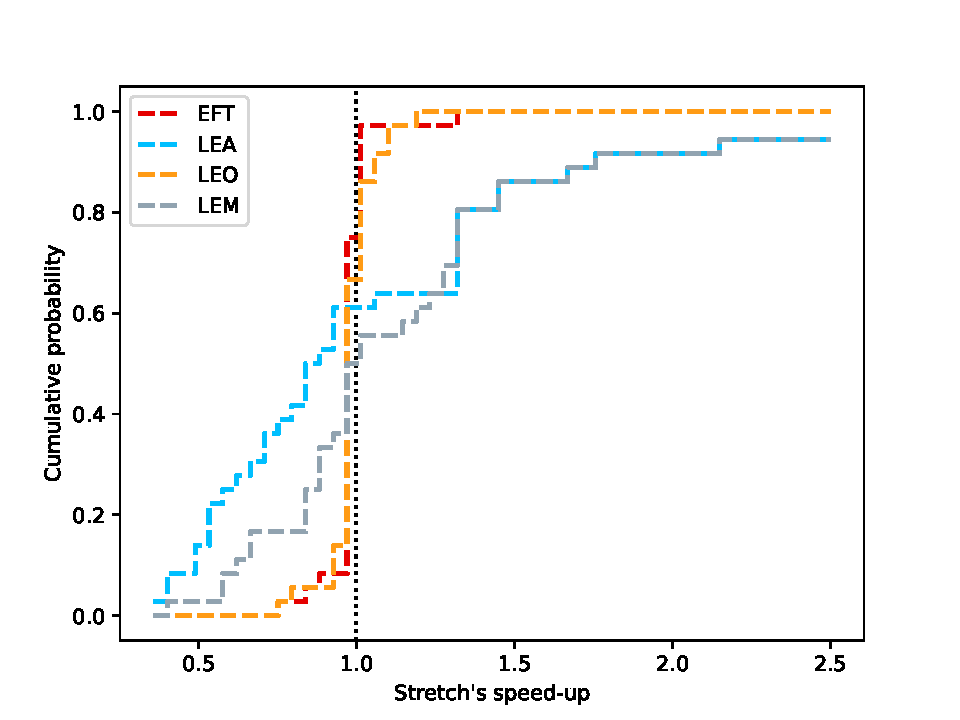
\includegraphics[width=1\linewidth]{../MBSS/plot/ECDF/ecdf_mean_stretch_all_workloads_bf.pdf}\caption{ECDF with backfilling}\end{figure}

\section{Conclusion}\label{sec.conclusion}

\todo[inline]{Max: 
Some schedulers do fairness as well with slurm or advance reservation with limitations (OAR).
We can tune our algorithms to do that as well.
Improve score to be efficient in any situation, any workload.
Improve mixed strategy to do more locality.}

\bibliographystyle{IEEEtran}
\bibliography{ref.bib}
\end{document}
